\subsubsection{Technology evolution and the Hype Cycle}\label{subsubsec:big-data--big-data--big-data-landscape-and-the-data-driven-value-cycle--technology-evolution-and-the-hype-cycle}

When a new technology appears, its adoption is rarely linear. A common pattern is:
\begin{equation*}
    \text{innovation}
    \rightarrow
    \text{hype}
    \rightarrow
    \text{disappointment}
    \rightarrow
    \text{maturity}
\end{equation*}
This is what the \definition{Hype Cycle} tries to describe. The important point is that the \hl{perceived importance of a technology and its real practical maturity are \textbf{not the same thing}.}

\highspace
A technology can be talked about everywhere, heavily funded, considered revolutionary, while still being technically immature or poorly understood.

\highspace
\begin{flushleft}
    \textcolor{Green3}{\faIcon{wave-square} \textbf{The basic shape}}
\end{flushleft}
The Hype Cycle is usually represented as a curve with:
\begin{equation*}
    x = \text{time}, \quad y = \text{expectations}
\end{equation*}
The typical progression is:
\begin{enumerate}
    \item \textbf{Technology Trigger}: a new technology appears, with prototypes and promising research results.
    \item \textbf{Peak of Inflated Expectations}: enthusiasm grows, and people start expecting the technology to solve almost everything.
    \item \textbf{Trough of Disillusionment}: reality catches up with expectations, and limitations become visible.
    \item \textbf{Slope of Enlightenment}: people start understanding what the technology is actually good for, and real use cases emerge.
    \item \textbf{Plateau of Productivity}: the technology becomes mature, and it reliably solves a known class of problems.
\end{enumerate}
Let's understand each phase.

\highspace
\begin{flushleft}
    \textcolor{Green3}{\faIcon{bolt} \textbf{1. Technology Trigger}}
\end{flushleft}
A new technology appears. At this point:
\begin{itemize}
    \item There may be prototypes;
    \item Research results are promising;
    \item Companies start experimenting;
    \item Practical use cases are still limited.
\end{itemize}
The technology is interesting, but not yet mature. For Big Data, this kind of \hl{phase happened when ideas} such as large-scale distributed data processing and new NoSQL systems \hl{began gaining attention.} The important thing is that the \hl{potential is high, but evidence is still limited.}

\highspace
\begin{flushleft}
    \textcolor{Green3}{\faIcon{rocket} \textbf{2. Peak of Inflated Expectations}}
\end{flushleft}
Then enthusiasm grows. People start expecting the technology to solve almost everything. We often hear claims such as: ``\emph{this will completely replace existing systems}'' or ``\emph{every company needs this}'' or ``\emph{this changes everything}''. Some early projects succeed, but \hl{many expectations are unrealistic}. This is the \important{hype} phase.

\highspace
For example, imagine a new database technology is introduced. Initially people may start saying: ``\emph{relation databases are obsolete}'' or ``\emph{every dataset should be moved to this new system}''. That is usually an \textbf{overreaction}. A new technology may be excellent for certain workloads without being universally superior.

\highspace
And this point is especially relevant in SMBUD. Later, when we see MongoDB, Cassandra, Redis, Neo4j, Elasticsearch, vector databases, we should \textbf{not} think:
\begin{equation*}
    \text{``newer technology''} = \text{``better technology''}
\end{equation*}
Instead: \hl{technology suitability depends on requirements.} For instance, a graph database is not ``\emph{better}'' than a relational database in general. It may be much better for relationship-heavy queries, while a relational DBMS may be more appropriate for another application.

\highspace
The Hype Cycle is therefore also a warning against \textbf{technology-driven design}. We should not choose a technology because it is fashionable.

\highspace
\begin{flushleft}
    \textcolor{Green3}{\faIcon{chart-line} \textbf{3. Trough of Disillusionment}}
\end{flushleft}
Eventually, \hl{reality catches up with expectations.} Projects fail. Limitations become visible. People discover problems such as: high operational complexity; scalability limits; poor tooling; expensive maintenance; missing features; difficult migration; lack of expertise.

\highspace
\hl{Enthusiasm then collapses.} The technology may suddenly look much less revolutionary. This is the \important{Trough of Disillusionment}. But this does \textbf{not necessarily mean that the technology is bad}. Instead, unrealistic expectations are being corrected.

\highspace
\begin{flushleft}
    \textcolor{Green3}{\faIcon[regular]{lightbulb} \textbf{4. Slope of Enlightenment}}
\end{flushleft}
At this stage, \textbf{people start understanding}: ``\emph{What is this technology actually good for?}''. Instead of saying: ``\emph{use it everywhere}''. The discussion becomes: ``\emph{use it when requirements X, Y, Z are present}''. Real use cases emerge. Best practices become clearer. Tooling improves. Companies gain operational experience. This is \hl{when the technology starts becoming genuinely useful.}

\highspace
\begin{flushleft}
    \textcolor{Green3}{\faIcon{check-circle} \textbf{5. Plateau of Productivity}}
\end{flushleft}
Eventually, the \hl{technology becomes mature.} It is no longer interesting because it is fashionable. It is \textbf{interesting because it reliably solves a known class of problems}. At this point: use cases are understood; benefits are measurable; limitations are known; tooling is mature; engineers know how to operate it. The technology has moved from \emph{hype} to \emph{engineering}. And that distinction is very important.

\begin{figure}[!htp]
    \centering
    \tikzsetnextfilename{hype-cycle}
    \tikzwidth{\linewidth}
    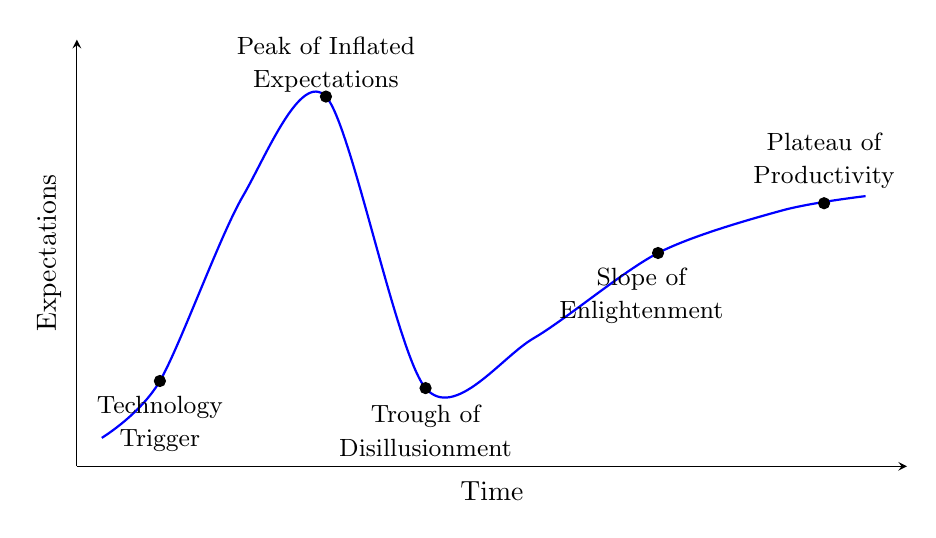
\begin{tikzpicture}
        \begin{axis}[
                width=\linewidth,
                height=7cm,
                axis lines=left,
                xlabel={Time},
                ylabel={Expectations},
                xmin=0, xmax=10,
                ymin=0, ymax=6,
                xtick=\empty,
                ytick=\empty,
                clip=false
            ]

            % Hype cycle curve
            \addplot[
                thick,
                smooth,
                blue,
            ] coordinates {
                (0.3,0.4)
                (1.0,1.2)
                (2.0,3.8)
                (3.0,5.2)
                (4.2,1.1)
                (5.5,1.8)
                (7.0,3.0)
                (8.5,3.6)
                (9.5,3.8)
            };

            % Key points
            \addplot[only marks, mark=*, mark size=2pt] coordinates {
                (1.0,1.2)
                (3.0,5.2)
                (4.2,1.1)
                (7.0,3.0)
                (9.0,3.7)
            };

            % Labels for phases
            \node[align=center] at (axis cs:1.0,0.6) {\small Technology\\\small Trigger};
            \node[align=center] at (axis cs:3.0,5.65) {\small Peak of Inflated\\\small Expectations};
            \node[align=center] at (axis cs:4.2,0.5) {\small Trough of\\\small Disillusionment};
            \node[align=center] at (axis cs:6.8,2.4) {\small Slope of\\\small Enlightenment};
            \node[align=center] at (axis cs:9.0,4.3) {\small Plateau of\\\small Productivity};

        \end{axis}
    \end{tikzpicture}
    \caption{\textbf{The Hype Cycle.} The curve represents the evolution of expectations over time for a new technology.}
    \label{fig:hype-cycle}
\end{figure}

\highspace
\begin{examplebox}[: NoSQL]
    Consider how people may react when NoSQL systems appear. At the beginning:
    \begin{center}
        ``\emph{Interesting alternative to relational databases}''
    \end{center}
    Then hype grows:
    \begin{center}
        ``\emph{SQL is dead!}''
    \end{center}
    Eventually problems emerge:
    \begin{itemize}
        \item limited joins
        \item weaker consistency in some systems
        \item application complexity
        \item data duplication
        \item operational challenges
    \end{itemize}
    So enthusiasm decreases. Later, the industry develops a more nuanced understanding:
    \begin{itemize}
        \item Cassandra is useful for certain distributed, write-heavy workloads.
        \item Neo4j is useful when relationships and graph traversals dominate.
        \item MongoDB is useful when document-oriented structures align well with the application.
        \item PostgreSQL remains excellent for many transactional systems.
    \end{itemize}
    This mature view is exactly what we want in SMBUD.
\end{examplebox}

\highspace
\begin{flushleft}
    \textcolor{Green3}{\faIcon{industry} \textbf{The connection with the Big Data market}}
\end{flushleft}
The reason the Hype Cycle appears right after the Big Data and AI market landscape is that \hl{markets around emerging technologies are extremely dynamic.} When a technological wave appears:
\begin{equation*}
    \text{new problem}
    \rightarrow
    \text{new technologies}
    \rightarrow
    \text{new companies}
    \rightarrow
    \text{huge expectations}
\end{equation*}
Many vendors enter the market. But some disappear, some merge, some technologies become standard, others remain niche, and others fail entirely. So the market landscape we saw earlier should not be interpreted as a fixed map. It \textbf{changes continuously as technologies mature}.

\highspace
\begin{flushleft}
    \textcolor{Green3}{\faIcon{question-circle} \textbf{Why this matters for a data engineer}}
\end{flushleft}
Imagine that our company says: ``\emph{Everyone is using vector databases. We should migrate everything to a vector database}''. A good engineer should \textbf{not answer}: ``\emph{Yes, because vector databases are modern}''. Instead, we ask:
\begin{equation*}
    \begin{aligned}
        &\text{What are our queries?}\\
        &\text{What type of data do we have?}\\
        &\text{What latency do we need?}\\
        &\text{What consistency guarantees?}\\
        &\text{What scale?}\\
        &\text{What problem are we solving?}
    \end{aligned}
\end{equation*}
Then we evaluate whether the technology fits those requirements. That is the engineering mindset the Hype Cycle encourages us to adopt.

\highspace
\begin{takeawaysbox}
    The \textbf{Hype Cycle} is essentially a model of the gap between \emph{expectations} and \emph{actual technological maturity}. The typical evolution is: (1) Trigger, (2) Inflated Expectations, (3) Disillusionment, (4) Understanding, (5) Productive Use.

    For us, the practical lesson is that \hl{we should not choose a technology because it is fashionable.} Instead, we should choose it because its \textbf{data model, architecture, and trade-offs fit the problem we are trying to solve.}
\end{takeawaysbox}
